\section{Romik's sofa}\label{app:romik}\label{sec:romik}

We describe Romik's shape \cite[Theorem~5]{Romik18} with its initial
contact point at $(1,1/2)$. This fixes the coordinates of the cap
$\KR$, hull $\HR$, and body $\SR$ used throughout the proof.

\subsection{The cubic and support coordinates}
The function $4y^3+3y$ is strictly increasing, is zero at $y=0$,
and exceeds one at $y=1$. Thus it has a unique positive root $Y$;
substitution gives $2/7<Y<3/10$. Set
\begin{equation}\label{eq:reference-parameters}
 \begin{aligned}
 \beta&=\arctan Y,&L&=\pi/2,\\
 A&=\frac1{4\sin\beta},&k&=1-\frac43A,\\
 T&=\frac32(\pi/4-\beta),&R&=\frac{\cos\beta}{\cos T}.
 \end{aligned}
\end{equation}
In particular $0<\beta<\pi/4$ and $\cos T>0$.
On $[0,L]$ define the two support coordinates
\begin{equation}\label{eq:reference-F}
 F(t)=\begin{cases}
 \cos t+\tfrac12\sin t,&0\le t\le\beta,\\
 R\cos(t/2+\pi/8)+k\cos t+\tfrac12\sin t,
       &\beta\le t\le L-\beta,\\
 (1-\tfrac23A)\cos t+\tfrac12\sin t+\tfrac12,
       &L-\beta\le t\le L,
 \end{cases}
\end{equation}
and
\begin{equation}\label{eq:reference-G}
 G(t)=\begin{cases}
 (2A-1)\sin t+\tfrac12\cos t+\tfrac12,&0\le t\le\beta,\\
 R\sin(t/2+\pi/8)-k\sin t+\tfrac12\cos t,
       &\beta\le t\le L-\beta,\\
 (\tfrac83A-1)\sin t+\tfrac12\cos t,
       &L-\beta\le t\le L.
 \end{cases}
\end{equation}

\begin{lemma}\label{lem:reference-matching}
The formulas for $F,G$ agree in value and first derivative at both
switches. They satisfy
\[
 F(0)=G(0)=F(L)=1,\qquad G(L)=\frac83A-1,
\]
and
\[
 F(L-t)=G(t)+2k\sin t,\qquad
 G(L-t)=F(t)-2k\cos t.
\]
\end{lemma}
\begin{proof}
Write $s=\sin\beta$ and $c=\cos\beta$. The matching identities
at the first switch are
\[
 R\cos(\beta/2+\pi/8)=\frac43A\cos\beta,
 \qquad R\sin(\beta/2+\pi/8)=\frac23,
 \qquad 4A\sin\beta=1.
\]
The cubic is precisely the angle-matching equation. Put
$\gamma=\beta/2+\pi/8$. Since $0<Y<1/3$, all the following
angles lie in the first tangent branch. The cubic gives
\[
 \frac{4Y}{1-4Y^2}=\frac{1+Y}{1-Y},
\]
so the double-angle and addition formulas yield
$2\arctan(2Y)=\beta+\pi/4$, or $\tan\gamma=2Y$.
Also $T=\pi/2-(\beta+\gamma)$, and therefore
\[
 \cos T=\sin\beta\cos\gamma+\cos\beta\sin\gamma
        =\tfrac32\cos\beta\sin\gamma.
\]
It follows that $R\sin\gamma=2/3$ and
$R\cos\gamma=1/(3Y)=(4A/3)\cos\beta$.
Substitution into
the first two phases proves agreement in value and first derivative
at $\beta$. The two complement
identities follow phase by phase from \cref{eq:reference-F,eq:reference-G}
and transfer matching to $L-\beta$. The endpoint values follow
directly.
\end{proof}

Define the half-plane pairs
\[
 \mathcal H_t=\{p:\ip{p}{u(t)}\le F(t),\
                    \ip{p}{u^\perp(t)}\le G(t)\}
 \quad(0\le t\le L),
\]
and then the hull and cap:
\begin{equation}\label{eq:reference-hull}
 \HR=\bigcap_{t\in[0,L]}(\mathcal H_t\cap\refl^{-1}\mathcal H_t),
 \qquad \KR=\HR^\downarrow.
\end{equation}
This definition makes convexity and reflection symmetry immediate.
At the axis normals it confines the hull to
$[1-8A/3,1]\times[0,1]$. The point $(k,1/2)$ satisfies the
half-plane inequalities, so the hull is nonempty and compact.

\begin{lemma}[Realization of the support coordinates]\label{lem:reference-support}
The hull $\HR$ is nonempty, compact, and convex. Its support values
at $t$ and $t+L$ are $F(t)$ and $G(t)$, respectively, for
$0\le t\le L$. Its upper boundary consists of the two arcs
\[
 B_F(t)=F(t)u(t)+F'(t)u^\perp(t),\qquad
 B_G(t)=G(t)u^\perp(t)-G'(t)u(t)
\]
and the segment joining them at the top normal.
\end{lemma}
\begin{proof}
Define an upper support $h$ on $[0,\pi]$ by
$h(t)=F(t)$ and $h(t+L)=G(t)$, and extend it to a periodic
function by $h(-t)=h(t)-\sin t$. The latter identity expresses
reflection in $y=1/2$. On each open phase its curvature radius is
\[
 \begin{array}{c|ccc}
  & (0,\beta)&(\beta,L-\beta)&(L-\beta,L)\\ \hline
  F''+F&0&\tfrac34R\cos(t/2+\pi/8)&\tfrac12\\
  G''+G&\tfrac12&\tfrac34R\sin(t/2+\pi/8)&0
 \end{array}
\]
All entries are nonnegative. Their middle-phase maximum is
$A\cos\beta=1/(4Y)<7/8$, by the matching identities and $Y>2/7$.
The one-sided derivatives of $h$ have an upward jump $4A/3$ at
$L$ and at $-L$, and no other jumps. Hence its curvature measure
$h\,\dd t+\dd h'$ is nonnegative.

Here is the support criterion directly in these coordinates.
For a smooth phase, the projection of its support point on a fixed
normal is $h(t)\cos(\phi-t)+h'(t)\sin(\phi-t)$, whose derivative is
\[
 \frac{\dd}{\dd t}\bigl(h(t)\cos(\phi-t)
                +h'(t)\sin(\phi-t)\bigr)
       =(h(t)+h''(t))\sin(\phi-t).
\]
As $t$ runs from $\phi-\pi$ to $\phi$, this projection increases,
and from $\phi$ to $\phi+\pi$ it decreases. At a derivative jump,
join the one-sided support points by the segment in the tangent
direction; its projected increments have the same sign. Every
point of the resulting closed curve therefore has projection at
most $h(\phi)$, and the support point at $\phi$ attains $h(\phi)$.
Taking its convex hull realizes all the half-planes defining $\HR$.
In particular $B_F(0)=(1,1/2)$ belongs to the hull, so it is
nonempty. The axis inequalities put it in the bounded rectangle
$[1-8A/3,1]\times[0,1]$; the half-plane intersection is closed,
and hence compact. The displayed arcs and the top segment give
its upper boundary.
\end{proof}

It follows that the projection and middle half are
\begin{equation}\label{eq:reference-projection}
 I_{\KR}=[1-8A/3,1],\qquad
 J_{\KR}=[1-2A,1-2A/3],\qquad w_{\KR}=8A/3.
\end{equation}
Indeed $B_F(L)=(1-2A/3,1)$ and $B_G(0)=(1-2A,1)$, since
$F'(L)=2A/3-1$ and $G'(0)=2A-1$. Thus the top segment is precisely
$J_{\KR}\times\{1\}$. The roof is one throughout $J_{\KR}$,
and reflection gives the bottom face over that interval. Convexity
therefore gives $J_{\KR}\times[0,1]\subset\HR$, so the hull has
nonempty interior.

\subsection{The niche and the two passages}

The supporting outer walls contain the hull at every angle. Removing
the points below both inner walls therefore gives a shape that passes
the corner. Removing the reflected niche gives the second passage. We
check that these two removals leave a connected band, so they describe
an admissible body.
Write $\nR=n_L(\HR)$, using the two-wall formula of
\cref{eq:niche}. Downward filling preserves upward support values,
so this is also $n_L(\KR)$. Define
\begin{equation}\label{eq:reference-sofa}
 \SR=\{(x,y)\in\HR:\nR(x)\le y\le1-\nR(x)\}.
\end{equation}
\begin{lemma}[The reference niche]\label{lem:reference-niche}
The niche $\nR$ is continuous, vanishes outside $J_{\KR}$,
and satisfies $0\le\nR(x)<1/2$ for every $x\in\R$.
\end{lemma}
\begin{proof}
Continuity follows from \cref{lem:barrier-continuity}. For confinement,
put $r_0=1-2A/3$ and $D(t)=1+r_0\cos t-F(t)$. At $L$,
$D(L)=D'(L)=0$, and
$D''+D=1-(F''+F)\ge0$. Solving this terminal-value equation gives
\[
 D(t)=\int_t^L[1-F(s)-F''(s)]\sin(s-t)\,\dd s\ge0.
\]
Consequently $F(t)-1\le r_0\cos t$, so $a_t(x)\le0$ whenever
$x\ge r_0$. The complement identities exchange the two walls
under $x\mapsto2k-x$, so $\nR(2k-x)=\nR(x)$. This gives the
same conclusion for $x\le1-2A$.

The height of the inner corner is
\[
 q_*(t)=(F(t)-1)\sin t+(G(t)-1)\cos t.
\]
Every two-wall minimum is at most this height: multiply its two
inequalities by $\sin^2t$ and $\cos^2t$ and add. In the first phase,
with $s=\sin\beta$,
\[
 q_*(t)-\tfrac12
   =\cos t\left(\frac{\sin t}{2s}-\frac12\right)-\sin t<0.
\]
The expression is negative at $t=0$ as well. In the middle phase,
with $z=t-\pi/4$,
\[
 q_*(t)-\tfrac12=R\cos(3z/2)-\sqrt2\cos z.
\]
Here $|z|\le\pi/4-\beta<\pi/6$, so
$\cos(3z/2)\le\cos z$ and $\cos z>0$.
Also $R=\cos\beta/\cos T<\sqrt2$, since $0<T<\pi/4$.
Thus this expression is negative. The last phase is the reflection
of the first. The continuous corner height therefore has a compact
maximum strictly below $1/2$, which bounds the entire niche.
\end{proof}

\begin{figure}[htbp]
 \centering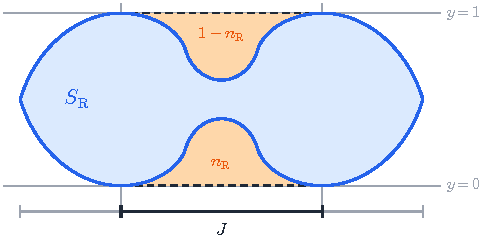
\includegraphics[width=.88\textwidth]{figures/fig-sofa.pdf}
 \caption{Romik's sofa is the hull (dashed) with the two open niches
 removed. Both niches lie over the middle half of the projection,
 and leave a positive band about $y=1/2$.}\label{fig:sofa}
\end{figure}

\begin{theorem}\label{thm:reference}
The set $\SR$ is an ambidextrous sofa of area $\Mc$ and
$\conv\SR=\HR$. It is invariant under reflection in $y=1/2$ and
is regular closed: $\clos(\inter\SR)=\SR$.
\end{theorem}
\begin{proof}
The set is closed in the compact hull. Every vertical fiber can be
joined within $\SR$ to the midline $y=1/2$, and the entire midline
segment over $I_{\KR}$ is present. This proves connectedness.
For the lower passage put $\phi=Lt$ and use the explicit placement
\begin{equation}\label{eq:reference-motion}
 p\longmapsto R_{-\phi}p+(1-F(\phi),1-G(\phi)),\qquad 0\le t\le1.
\end{equation}
The outer supporting half-planes give the two outer wall constraints.
The niche inequality gives the inner-corner alternative at every
interior angle. At $t=0$ the placement is the identity and the sofa
lies in $\Hin$; at $t=1$ it is
$(x,y)\mapsto(y,2-8A/3-x)$, which lies in $\Vm$ by the projection
and strip bounds. Reflection gives the upper passage with angle
$\phi$ and the same initial placement.

The boundary support points of $\HR$ survive the niche trimming.
The upper boundary arcs have abscissae outside the interior of the
top interval, where the niche is zero; their reflected arcs give
the remaining supports. Thus $\SR$ has the same
support function as $\HR$, which proves the convex-hull identity.
Finally the continuous strict niche band and the interior of the
hull approximate every boundary point from inside $\SR$. At points
on either niche boundary, a small displacement toward the midline
gives the approximation; the strict $1/2$ margin preserves the other
constraint. This proves regular closedness.

The area calculation follows below.
\end{proof}

\subsection{Exact value}
The value is obtained from the support functional $\mathcal A$
of \cref{sec:calibration}, before any optimality theorem is used.
For the reference pair, integration by parts in its Euler equations
evaluates the functional without integrating its algebraic boundary.
Put $p=F'-G+1$ and $q=G'+F-1$. On the first phase,
\[
 p=\tfrac12-2A\sin t,\qquad q=2A\cos t-1;
\]
on the middle phase, with $\varphi=t/2+\pi/8$,
\[
 p=1-\tfrac32R\sin\varphi,\qquad
 q=\tfrac32R\cos\varphi-1.
\]
The last phase is obtained by $p(L-t)=-q(t)$.
Thus $p\ge0$ on $[0,\beta]$ and $p\le0$ on $[\beta,L]$;
$q\ge0$ on $[0,L-\beta]$ and $q\le0$ afterwards.
At the switches $p(\beta)=q(L-\beta)=0$.

The Euler equations of \cref{eq:support-functional} on the three
phases are, respectively,
\[
 F''+F=0,\quad G''+G=\tfrac12;
\]
\[
 2F''-G'+F=0,\quad 2G''+F'+G=0;
\]
\[
 F''+F=\tfrac12,\quad G''+G=0.
\]
The displayed formulas for $F,G$ satisfy them by differentiation.
The two derivative fluxes are
\[
 J_F=-F'-(G-1)/2-p_-,\qquad
 J_G=-G'+(F-1)/2-q_+.
\]
They are continuous across both switches because the corresponding
contact momentum vanishes there. Their endpoint values are
\[
 J_F(0)=-\tfrac12,\quad J_G(0)=2-4A,
 \qquad J_F(L)=1,\quad J_G(L)=\tfrac12.
\]
Integration by parts therefore gives
\[
 D\mathcal A(F,G)[F,G]
   =[J_FF+J_GG]_0^L=\frac{16}3A-1.
\]
If $A_X$ denotes the functional density and $D_X$ its
self-variation density, expansion gives
\[
 2A_X-D_X=2-F-G+(F'-G')/2-p_-+q_+.
\]
Primitives of this remainder on the three phases are
\begin{align*}
 V_1(t)&=t/2+(2A-1/4)\cos t+(A-3/4)\sin t,\\
 V_2(t)&=(G(t)-F(t))/2,\\
 V_3(t)&=t/2-(1/4-A/3)\cos t-(3/4+2A/3)\sin t.
\end{align*}
Differentiating each primitive, with the corresponding contact
signs, verifies the remainder. Summing their increments and using
the matching values gives
\[
 2\mathcal A(F,G)-D\mathcal A(F,G)[F,G]
       =4A\cos\beta-\frac83A-1+\beta.
\]
Consequently
\begin{equation}\label{eq:reference-functional-value}
 \begin{aligned}
 \mathcal A(F,G)&=\frac43A+2A\cos\beta-1+\frac\beta2,\\
 P_L(\KR)&=\mathcal A(F,G)-\frac{w_{\KR}}2
          =2A\cos\beta-1+\frac\beta2.
 \end{aligned}
\end{equation}
For the second equality, \cref{lem:cap-support-area} expresses
the cap area by its support energy. The curvature bounds,
contact signs, and top face established above verify all the
hypotheses of \cref{cor:horizontal-score-identity}; its signed
graph calculation identifies the niche integral. This uses only
the reference geometry, independently of any optimality conclusion.

Since $4A\cos\beta=\cot\beta=1/Y$ and the cubic gives
$1/Y=4Y^2+3$, \cref{eq:reference-functional-value} yields
$P_L(\KR)=\Mc/2$. Cavalieri's principle now gives the body's area.
Outside $J_{\KR}$ the niche is zero; on $J_{\KR}$ the hull fills
the full unit-height fiber. Hence
\[
 \abs{\SR}
  =2\abs{\KR}-w_{\KR}-2\int_{J_{\KR}}\nR
  =2P_L(\KR)=\Mc.
\]


For comparison with Romik's closed form, put
$a=\sqrt[3]{\sqrt2+1}$ and $b=\sqrt[3]{\sqrt2-1}$, so $ab=1$.
Expansion shows that $Y=(a-b)/2$ solves the cubic and is positive.
Also
$1+4Y^2=a^2+b^2-1$. Therefore
\begin{equation}\label{eq:romik-radicals}
 \Mc=\sqrt[3]{3+2\sqrt2}+\sqrt[3]{3-2\sqrt2}-1
       +\arctan\!\left(\frac{\sqrt[3]{\sqrt2+1}
                            -\sqrt[3]{\sqrt2-1}}2\right).
\end{equation}
